\documentclass[tikz,border=7pt]{standalone}
\usepackage{amsmath,amssymb}
\usetikzlibrary{arrows.meta,backgrounds,fit,positioning}

\definecolor{stateblue}{HTML}{0072B2}
\definecolor{actionorange}{HTML}{E69F00}
\definecolor{riskgreen}{HTML}{009E73}
\definecolor{futurepurple}{HTML}{CC79A7}
\definecolor{ink}{HTML}{222222}
\definecolor{muted}{HTML}{666666}
\definecolor{panel}{HTML}{F4F7F9}

\tikzset{
  flow/.style={-{Stealth[length=2.2mm]}, line width=0.8pt, draw=ink},
  feedback/.style={-{Stealth[length=2.2mm]}, line width=0.8pt, draw=stateblue, dashed},
  block/.style={
    rounded corners=2mm,
    draw=ink,
    line width=0.8pt,
    fill=white,
    minimum height=22mm,
    text width=34mm,
    align=center,
    inner sep=3mm,
    font=\sffamily\small
  },
  state/.style={block, draw=stateblue, line width=1.2pt},
  action/.style={block, draw=actionorange, line width=1.2pt},
  risk/.style={block, draw=riskgreen, line width=1.2pt},
  future/.style={
    block,
    draw=futurepurple,
    dashed,
    fill=futurepurple!4,
    minimum height=17mm
  },
  note/.style={
    rounded corners=1.5mm,
    draw=muted,
    fill=panel,
    text width=33mm,
    align=center,
    inner sep=2.5mm,
    font=\sffamily\footnotesize
  }
}

\begin{document}
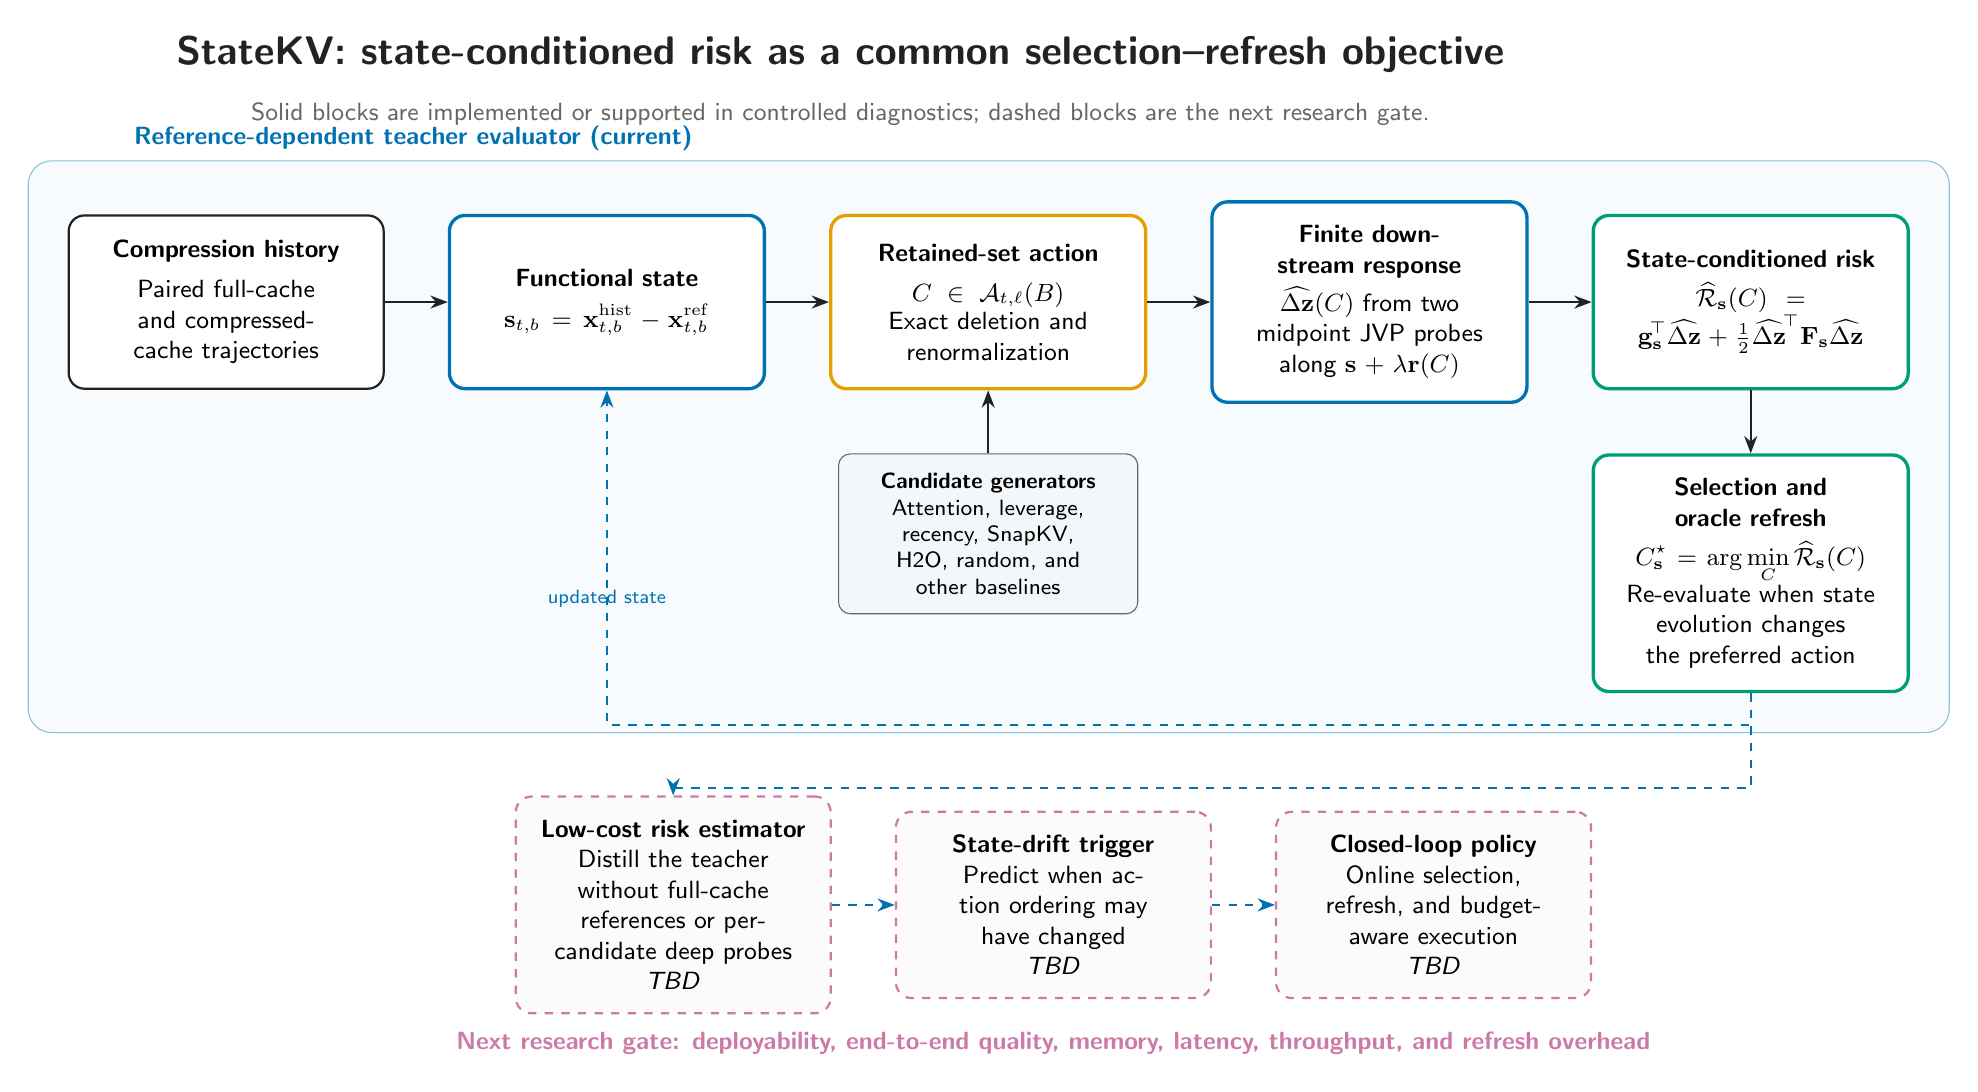
\begin{tikzpicture}[node distance=8mm and 8mm]
  \node[font=\sffamily\bfseries\Large, text=ink] (title)
    {StateKV: state-conditioned risk as a common selection--refresh objective};
  \node[font=\sffamily\small, text=muted, below=1.5mm of title] (subtitle)
    {Solid blocks are implemented or supported in controlled diagnostics; dashed blocks are the next research gate.};

  \node[block, below=10mm of subtitle, xshift=-78mm] (history) {
    \textbf{Compression history}\\[1.2mm]
    Paired full-cache and compressed-cache trajectories
  };
  \node[state, right=of history] (state) {
    \textbf{Functional state}\\[1.4mm]
    $\displaystyle \mathbf{s}_{t,b}=\mathbf{x}^{\mathrm{hist}}_{t,b}-\mathbf{x}^{\mathrm{ref}}_{t,b}$
  };
  \node[action, right=of state] (action) {
    \textbf{Retained-set action}\\[1.2mm]
    $\displaystyle C\in\mathcal{A}_{t,\ell}(B)$\\[-0.2mm]
    Exact deletion and renormalization
  };
  \node[state, right=of action] (response) {
    \textbf{Finite downstream response}\\[1.0mm]
    $\widehat{\Delta\mathbf z}(C)$ from two midpoint JVP probes along $\mathbf{s}+\lambda\mathbf r(C)$
  };
  \node[risk, right=of response] (risk) {
    \textbf{State-conditioned risk}\\[1.0mm]
    $\displaystyle \widehat{\mathcal R}_{\mathbf s}(C)
      =\mathbf g_{\mathbf s}^{\!\top}\widehat{\Delta\mathbf z}
      +\tfrac12\widehat{\Delta\mathbf z}^{\!\top}\mathbf F_{\mathbf s}\widehat{\Delta\mathbf z}$
  };

  \draw[flow] (history) -- (state);
  \draw[flow] (state) -- (action);
  \draw[flow] (action) -- (response);
  \draw[flow] (response) -- (risk);

  \node[note, below=8mm of action] (candidates) {
    \textbf{Candidate generators}\\
    Attention, leverage, recency, SnapKV, H2O, random, and other baselines
  };
  \draw[flow] (candidates) -- (action);

  \node[risk, below=8mm of risk] (decision) {
    \textbf{Selection and oracle refresh}\\[1.1mm]
    $\displaystyle C^{\star}_{\mathbf s}=\arg\min_C\widehat{\mathcal R}_{\mathbf s}(C)$\\[-0.2mm]
    Re-evaluate when state evolution changes the preferred action
  };
  \draw[flow] (risk) -- (decision);
  \draw[feedback] (decision.south) -- ++(0,-4mm) -|
    node[pos=0.66, above, font=\sffamily\scriptsize, text=stateblue]
    {updated state} (state.south);

  \begin{scope}[on background layer]
    \node[rounded corners=3mm, draw=stateblue!45, fill=stateblue!3,
      fit=(history)(state)(action)(response)(risk)(candidates)(decision),
      inner sep=5mm, label={[font=\sffamily\bfseries\small, text=stateblue]above left:Reference-dependent teacher evaluator (current)}] {};
  \end{scope}

  \node[future, below=23mm of candidates, xshift=-40mm] (distill) {
    \textbf{Low-cost risk estimator}\\
    Distill the teacher without full-cache references or per-candidate deep probes\\
    \emph{TBD}
  };
  \node[future, right=of distill] (drift) {
    \textbf{State-drift trigger}\\
    Predict when action ordering may have changed\\
    \emph{TBD}
  };
  \node[future, right=of drift] (online) {
    \textbf{Closed-loop policy}\\
    Online selection, refresh, and budget-aware execution\\
    \emph{TBD}
  };
  \draw[feedback] (distill) -- (drift);
  \draw[feedback] (drift) -- (online);
  \draw[feedback] (decision.south) -- ++(0,-12mm) -| (distill.north);

  \node[font=\sffamily\bfseries\small, text=futurepurple, below=3mm of drift]
    {Next research gate: deployability, end-to-end quality, memory, latency, throughput, and refresh overhead};
\end{tikzpicture}
\end{document}
